\chapter{Design architetturale}

\section{Pattern architetturali}
L’architettura del sistema è una classica \textbf{Client-Server}. \\
La parte server è stata suddivisa in \textbf{microservizi RESTFul}, a basso coupling, per aumentare la modularità;
\\
Il lato Server è stato realizzato secondo i principi della \textbf{Clean Architecture}, un pattern architetturale utile per ottenere una buona separazione dei compiti. 
\\
Il client adopera inoltre un'architettura \textbf{Component-Based}.
\subsection{Clean Architecture}
Per ottenere la separazione dei compiti, tale architettura impone la suddivisione del codice in differenti strati: ogni strato
può conoscere, chiamare ed utilizzare solo gli strati più interni, imponendo così la \textit{Dependency Rule}: in tal modo i cambiamenti di codice in uno strato esterno non causano modifiche agli strati interni. La Dependency Rule permette, dunque, di creare un sistema 
intrinsecamente modificabile e testabile, con tutti i benefici che ciò comporta. Inoltre, seguendo il \textit{Single Responsability Principle} e
dipendendo solo da astrazioni, diventa semplice sostituire le implementazioni.
\\

\begin{figure}
  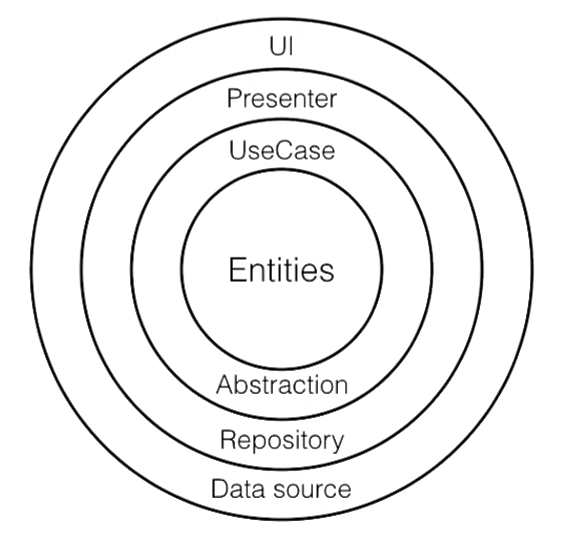
\includegraphics[scale=0.5, center]{images/CleanArchitectureLayersWhite.png}
  \caption{Rappresentazione della Dependency Rule e degli strati della Clean Architecture.}
  \label{fig: clean-architecture-layers-white}
\end{figure}

\begin{figure}
  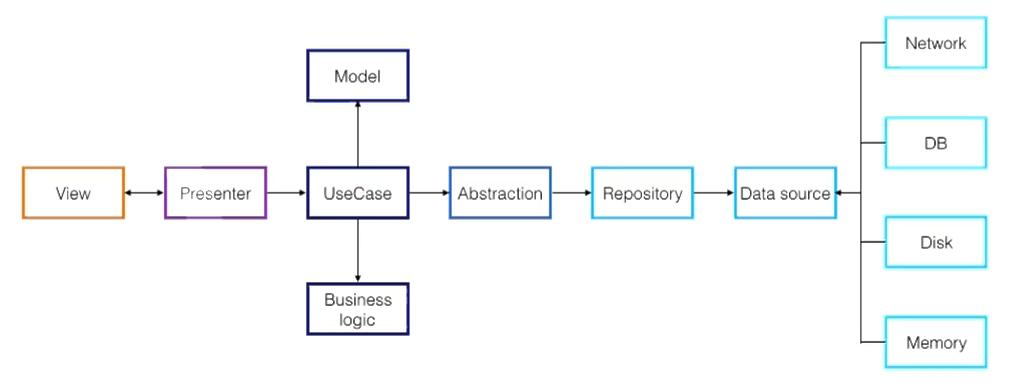
\includegraphics[width=\linewidth]{images/CleanArchitectureFlowWhite.png}
  \caption{Diagramma contenente tutti gli strati della Clean Architecture e le loro relazioni}
  \label{fig: clean-architecture-flow-white}
\end{figure}

Gli strati che compongono l'architettura sono i seguenti:
\begin{itemize}
    \item \textit{View}: prende gli eventi utente e li passa al presenter, mostrando inoltre i dati ricevuti dal presenter e permettendo
    azioni relative all'interfaccia grafica, come la gestione delle animazioni;
    \item \textit{Presenter}: fa da "middle man" tra la View e gli Use Cases; è il Presenter che formatta e passa i dati da visualizzare alla view e che gestisce gli eventi utente in arrivo dalla view, chiamando poi il giusto Use Case. Nel codice del Presenter non bisogna inserire nulla di relativo ad un singolo framework, poichè deve essere indipendente da essi;
    \item \textit{Use Case}: sono classi contenenti la logica necessaria per implementare un use case, ovvero uno specifico compito di business che l'utente cerca di portare a termine. Gli Use Case adoperano le classi di \textit{Model} e sfruttano uno o più abstractions. Dunque, gli Use Cases 
    ottengono i dati tramite le abstractions; a seguito di ciò essi usano le più appriopriate classi di business logic, per poi restituire un risultato, in modo asincrono, tramite un \textit{Subscriber} che il Presenter ha fornito;
    \item \textit{Abstraction}: astrazione per componenti specifici ad un framework;
    \item \textit{Repository}: un Repository è un data provider; al suo interno si sceglie quale \textit{Data Store} usare o, in caso se ne usi più di uno in contemporanea, se ne unisce i risultati (ad esempio si sceglie la sorgente dati che per prima restituisce il risultato). Il repository mappa in modo opportuno il risultato ottenuto, in modo che sia comprensibile dagli strati superiori, facendone in caso anche caching.
     \item \textit{Data Store}: è un'implementazione di una specifica sorgente dati; è dunque possibile realizzare multipli Data Source, uno per ogni tipologia di sorgente dati: Internet, Database, Disco Rigido, Memoria Centrale.
\end{itemize}
Il primo strato, ovvero la View, non è presente lato Server, poichè è il Client che se ne occupa.
\\
\\
La Clean Architecture permette di
ottenere i migliori risultati se usata assieme ai seguenti elementi, i quali sono stati da noi adottati:
\begin{itemize}
\item Un framework o tecnica di \textit{Dependency Injection}, per estrarre il codice di creazione delle dipendenze dalle classi, ottenendo codice più riusabile, testabile, leggibile e con maggiore separazione dei compiti. Qui la scelta è ricaduta sul \textit{Constructor Injection}, per la sua immediatezza nell'utilizzo;
\item \textit{Reactive Extensions}, per operare su sequenze di dati asincroni in modo dichiarativo e funzionale;
\item Un ampio uso delle lambdas, per ridurre la quantità di codice boilerplate.
\end{itemize}

\subsection{Microservizi}
Per architettura a microservizi si intende un'architettura formata da una collezione di servizi tra loro cooperanti e debolmente accoppiati, ovvero che non richiedono uno stack tecnologico specifico per l'interoperabilità, a meno delle principali tecnologie web. 
\\Il beneficio principale della scomposizione di un unico software monolite in più servizi è l'aumento di modularità, rendendo così più facile lo sviluppo: infatti, tale architettura permette di sviluppare e testare parti più piccole del sistema. Inoltre, permette lo sviluppo in maniera parallela e autonoma da parte di più teams. \\Infine, questa architettura rende più facile il raggiungimento di un buon livello di resilienza e scalabilità,  poichè, in caso di bisogno di replicazione, è possibile replicare la sola parte interessata, senza dover replicare l'intero monolite; infatti, spesso parti diverse del monolite hanno caratteristiche e necessità diverse, dunque è giusto permettere ad ogni parte di essere ridondata in un numero corretto di volte.

\subsection{Architettura del Client}
Il client è stato realizzato secondo un'architettura \textit{Component-Based}, che comprende i seguenti elementi:
\begin{itemize}
    \item \textit{Template}: definisce come renderizzare un componente, specificandone gli elementi grafici e i data bindings (mono o bidirezionali) dei relativi dati;
    \item \textit{Component}: è il codice che gescisce una sezione della vista, aggiornandone i dati e reagendo agli eventi, 
    chiamando, se necessario, uno o più \textit{Services}. Un Component è sempre associato ad un template. 
    I vari Component si distribuiscono ad albero, infatti ogni component può a sua volta contenere ulteriori Components, formando così la struttura della view.
    \item \textit{Service}: è un'ampia categoria che comprende un qualsiasi valore, funzione o funzionalità di cui l'applicazione ha bisogno.
\end{itemize}
Infine, è stato fatto abbondante uso di \textit{Dependency injection} sia nei Components sia nei Services, tramite i loro costruttori.

\section{Componenti del sistema distribuito}
Come già introdotto nella sezione precedente, il sistema vuole realizzare una \textit{Web Application} basata sul classico modello architetturale Client-Server.
Mentre la parte Client del sistema è rappresentata da un'unica applicazione monolitica, il sistema Server è stato scomposto in più componenti seguendo il modello a microservizi.
Dopo una prima fase di design del back-end del sistema, sono stati identificati 4 microservizi principali:
\begin{itemize}
    \item \textit{WebApp Service}
    \item \textit{User Service}
    \item \textit{Room Service}
    \item \textit{Authentication Service}
\end{itemize}
Inoltre è stato successivamente introdotto anche un \textit{servizio di Heartbeat} per permettere lo sviluppo della feature di visualizzazione dello stato effettivo di connessione al sistema di un utente.
Infine, viene descritta la struttura dei \textit{DB} utilizzati da ogni microservizio ai fini della persistenza delle informazioni.
Prima di descrivere ogni componente, viene successivamente definito il modello di riferimento delle entità di business del sistema. La definizione di tale modello infatti impatterà la struttura dei dati utilizzata da ogni componente.

\subsection{Model}
Prima di addentrarsi nell'analisi di ogni singolo componente del sistema distribuito, sono stati modellati i concetti di business principali tramite un diagramma delle classi \textit{UML}. Questa fase sarà utile poi per il design di ogni componente poichè permette di definire lo schema di base della struttura dei dati. Le entità di dominio e le relative associazioni sono espresse in Figura \ref{fig:model-class-diagram}.
\begin{figure}
  \centering
  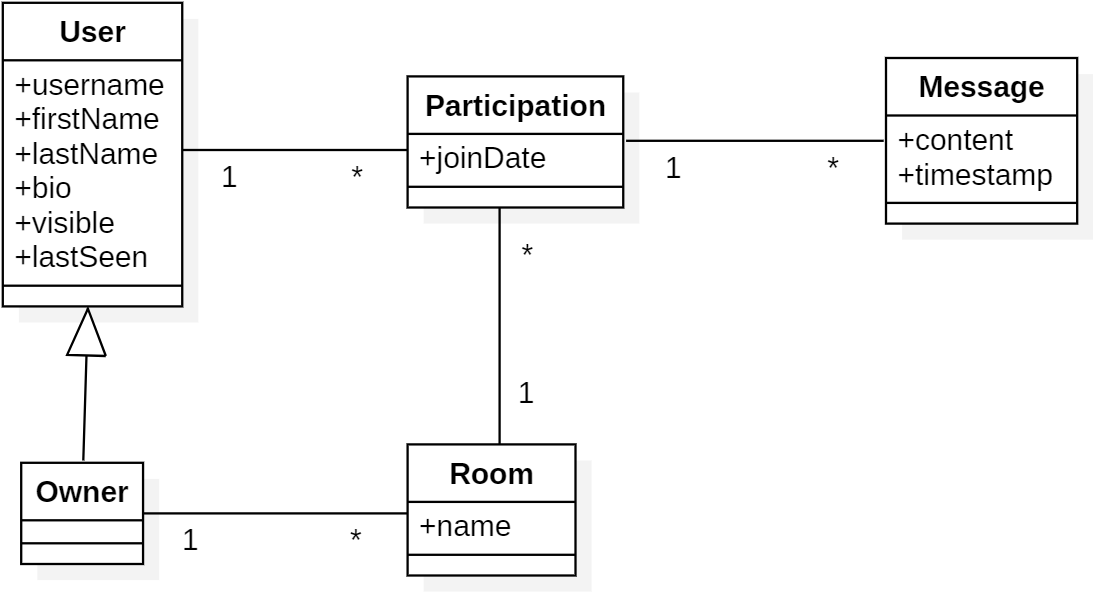
\includegraphics[height=15cm, width=12cm,
		keepaspectratio]{images/ModelClassDiagram.png}
  \caption{Diagramma delle classi delle entità di business.}
  \label{fig:model-class-diagram}
\end{figure}

\subsection{Web Client}
Rappresenta la parte del sistema utilizzabile dall'utente tramite un browser. Questo componente permette la visualizzazione delle schermate tramite le quali l'utente può interagire col sistema ed effettuare tutte le operazioni di business definite in fase di analisi del problema. Il \textit{Web Client} interagisce con il \textit{Server} sia in maniera \textit{pull} sia in maniera \textit{push}: questa duplice modalità di interazione permette di creare un sito web reattivo ai cambiamenti in maniera efficiente. Non vi è infatti, la necessità di effettuare \textit{polling} sul server per verificare se i dati sono stati aggiornati.
Nelle seguenti sottosezioni vengono definiti i componenti del sistema \textit{Client} considerando le astrazioni fornite dal framework \textit{Angular}.
\subsubsection{Components}
I principali componenti \textit{Angular} del \textit{front-end} identificati sono:
\begin{itemize}
    \item \textit{\textbf{Registration}}: incapsula la grafica della schermata di registrazione di un utente e la logica di controllo degli eventi scatenati dalla relativa interfaccia.
    \item \textit{\textbf{Login}}: incapsula la grafica della schermata di login e la logica di controllo degli eventi scatenati dalla relativa interfaccia.
    \item \textit{\textbf{Add-room}}: incapsula la grafica della schermata di creazione di una stanza e la logica di controllo degli eventi scatenati dalla relativa interfaccia.
    \item \textit{\textbf{Edit-profile}}: incapsula la grafica della schermata di \textit{editing} del proprio profilo utente, la logica di controllo degli eventi scatenati dalla relativa interfaccia e l'attivazione del recupero delle informazioni dell'utente corrente.
    \item \textit{\textbf{Room-info}}: incapsula la grafica della schermata di visualizzazione delle informazioni di una stanza, la logica di controllo degli eventi scatenati dalla relativa interfaccia e l'attivazione del recupero delle informazioni della stanza selezionata.
    \item \textit{\textbf{Rooms}}: incapsula la grafica della lista delle stanze a cui l'utente si è unito, la logica di controllo degli eventi scatenati dalla relativa interfaccia e l'attivazione del recupero delle stanze.
    \item \textit{\textbf{Search-rooms}}: incapsula la grafica della lista delle stanze ricercate, la logica di controllo degli eventi scatenati dalla relativa interfaccia e l'attivazione del recupero delle stanze. 
    \item \textit{\textbf{Sidebar}}: incapsula la grafica della schermata di visualizzazione delle stanze cercate o a cui l'utente si è unito e la logica di controllo degli eventi scatenati dalla relativa interfaccia.
    \item \textit{\textbf{Top-navbar}}: incapsula la grafica della barra di navigazione e la logica di controllo degli eventi scatenati dalla relativa interfaccia.
    \item \textit{\textbf{User-profile}}: incapsula la grafica della schermata di visualizzazione del profilo di un utente e l'attivazione del recupero delle informazioni sull'utente visualizzato.
\end{itemize}
\subsubsection{Services}
I servizi \textit{Angular} identificati sono:
\begin{itemize}
    \item \textit{\textbf{Authentication}}: mantiene il riferimento all'utente che si è autenticato e fornisce le funzionalità di \textit{login}, \textit{registrazione}, \textit{logout}.
    \item \textit{\textbf{Chat}}: permette di effettuare le principali chiamate, riguardanti la \textit{Chat}, al \textit{Server} e di intercettarne le relative risposte in maniera asincrona. 
    \item \textit{\textbf{User}}: offre le funzionalità di recupero/modifica del profilo utente e permette di aggiornare le informazioni sullo stato di connessione del \textit{Client}.
    \item \textit{\textbf{Event-bus}}: permette di utilizzare l'\textit{Event Bus} di \textit{Vertx} per interagire in maniera non bloccante secondo il modello \textit{publish-subscribe}. Viene utilizzato per intercettare gli eventi asincroni provenienti dal \textit{Server}. 
\end{itemize}

\subsubsection{Template}
Il template di base del front-end è la versione di \href{https://startangular.com/product/sb-admin-material/}{\textit{\underline{SB Admin}}} realizzata tramite componenti dell'UI framework \textit{Angular Material}. Sono stati utilizzati alcuni componenti del predetto template, editandoli in maniera opportuna per addattarli alle nostre esigenze grafiche. L'utilizzo di tale framework ha permesso di creare uno sito web accessibile e  naturalmente \textit{responsive}.
In Figura \ref{fig:sb-admin-login} viene mostrata la schermata iniziale del template precedentemente citato.
\begin{figure}
  \centering
  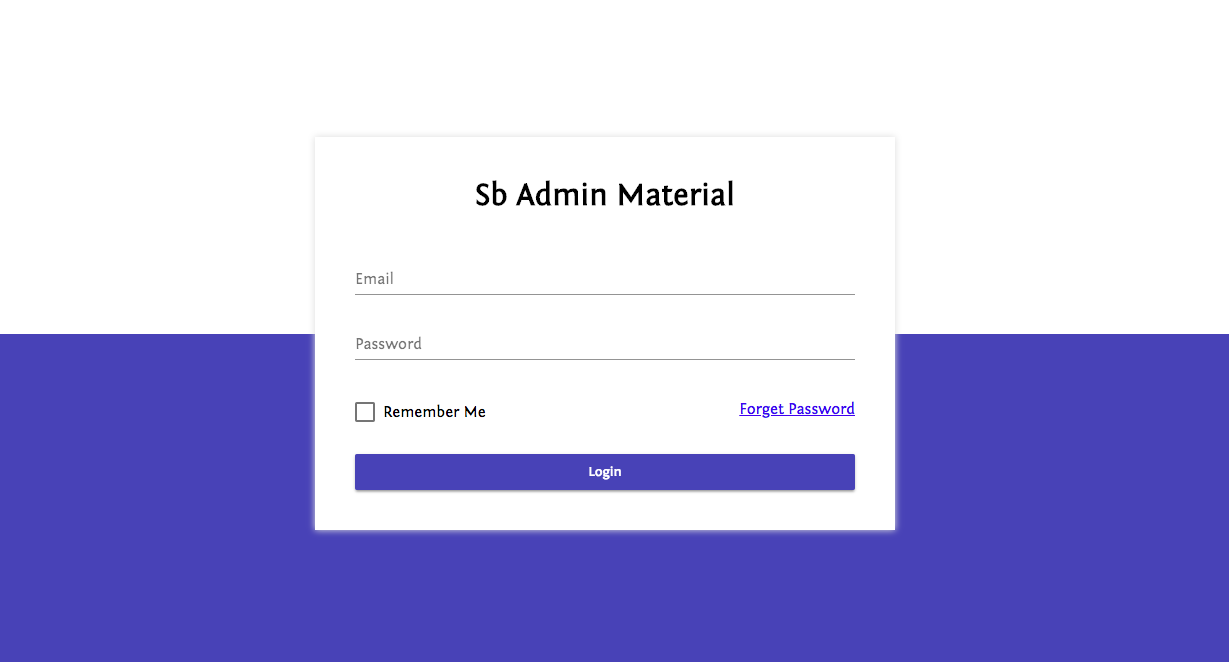
\includegraphics[height=15cm, width=12cm,
		keepaspectratio]{images/sb-admin.png}
  \caption{Schermata di login del template SB Admin realizzato tramite il framework UI \textit{Angular Material}.}
  \label{fig:sb-admin-login}
\end{figure}

\subsection{Web Server}
\subsubsection{Struttura}
Si elencano e descrivono di seguito, i componenti nei quali il \textit{Web Server} è stato scomposto. Come detto in precedenza infatti, questa parte del sistema è stata progettata secondo il modello a microservizi. 

\paragraph{WebApp Service}
Il \textit{WebApp Service} rappresenta il microservizio che gestisce l'interazione tra il client ed i restanti servizi di back-end. Il suo ruolo principale è quello di intercettare le richieste da parte dei client ed eseguire le operazioni necessarie per elaborare e restituire il relativo risultato. Nel perseguire il suo obiettivo il \textit{WebApp Service} tipicamente interagisce con uno o più microservizi di back-end.
La struttura del \textit{WebApp Service} è descritta tramite un diagramma UML delle classi in Figura \ref{fig:webapp-service-class-diagram}. In tale figura sono stati omessi alcuni dei casi d'uso per facilitare la lettura del resto del diagramma. Per completezza, si riporta la lista completa dei casi d'uso del \textit{WebApp Service} e le relative associazioni ai repositories:
\begin{itemize}
    \item \textit{\textbf{LoginUserUseCase}} $\longrightarrow$ \textit{AuthenticationRepository}, \textit{UserRepository}
    
    \item \textit{\textbf{RegisterUserUseCase}} $\longrightarrow$ \textit{AuthenticationRepository}, \textit{UserRepository}, \textit{RoomRepository}
    
    \item \textit{\textbf{LogoutUserUseCase}} $\longrightarrow$ \textit{AuthenticationRepository}, \textit{UserRepository}
    
    \item \textit{\textbf{JoinRoomUseCase}} $\longrightarrow$ \textit{AuthenticationRepository}, \textit{RoomRepository}
    
    \item \textit{\textbf{LeaveRoomUseCase}} $\longrightarrow$ \textit{AuthenticationRepository}, \textit{RoomRepository}
    
    \item \textit{\textbf{NotifyTypingInRoomUseCase}} $\longrightarrow$ \textit{AuthenticationRepository}
    
    \item \textit{\textbf{SendMessageUseCase}} $\longrightarrow$ \textit{AuthenticationRepository}, \textit{RoomRepository}
    
    \item \textit{\textbf{GetUserUseCase}} $\longrightarrow$ \textit{AuthenticationRepository}, \textit{UserRepository}
    
    \item \textit{\textbf{GetUserParticipationsUseCase}} $\longrightarrow$ \textit{AuthenticationRepository}, \textit{RoomRepository}
    
    \item \textit{\textbf{GetRoomsUseCase}} $\longrightarrow$ \textit{AuthenticationRepository}, \textit{RoomRepository}
    
    \item \textit{\textbf{GetRoomParticipationsUseCase}} $\longrightarrow$ \textit{AuthenticationRepository}, \textit{RoomRepository}
    
    \item \textit{\textbf{GetMessagesUseCase}} $\longrightarrow$ \textit{AuthenticationRepository}, \textit{RoomRepository}
    
    \item \textit{\textbf{EditUserUseCase}} $\longrightarrow$ \textit{AuthenticationRepository}, \textit{UserRepository}
    
    \item \textit{\textbf{DeleteRoomUseCase}} $\longrightarrow$ \textit{AuthenticationRepository}, \textit{RoomRepository}
    
    \item \textit{\textbf{CreateRoomUseCase}} $\longrightarrow$
    \textit{AuthenticationRepository}, \textit{RoomRepository}
    
    \item \textit{\textbf{UserOfflineUseCase}} $\longrightarrow$ \textit{UserRepository}
\end{itemize}

\begin{figure}
  \centering
  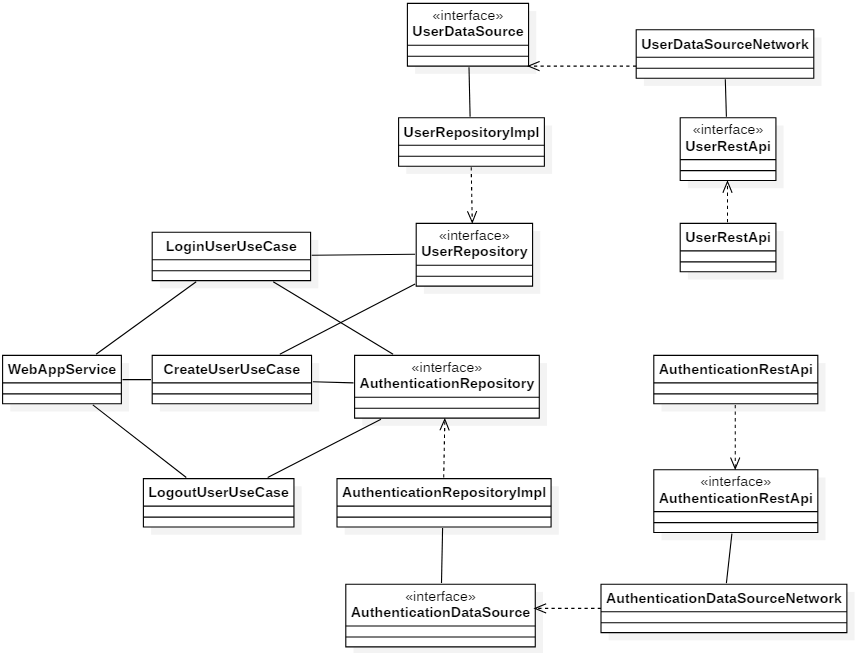
\includegraphics[height=15cm, width=12cm,
		keepaspectratio]{images/WepAppServiceClassDiagram.png}
  \caption{Diagramma delle classi dell'\textit{WebApp Service} (alcuni casi d'uso sono stati omessi per facilitare la lettura dello schema).}
  \label{fig:webapp-service-class-diagram}
\end{figure}

\paragraph{User Service}
Lo \textit{User Service} è il servizio che si occupa della persistenza delle informazioni degli utenti. Offre le classiche operazioni di lettura, scrittura ed aggiornamento sui dati utente. Esempi di operazioni che coinvolgono il servizio sono: reperimento della biografia utente, modifica del nome e cognome, ecc.
\begin{figure}
  \centering
  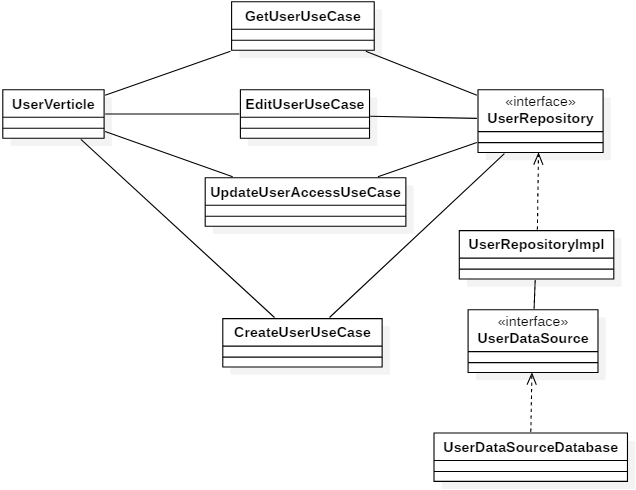
\includegraphics[height=15cm, width=12cm,
		keepaspectratio]{images/UserServiceClassDiagram.png}
  \caption{Diagramma delle classi dell'\textit{User Service}.}
  \label{fig:user-service-class-diagram}
\end{figure}

\paragraph{Room Service}
Il \textit{Room Service} è il servizio che si occupa della persistenza delle informazioni delle stanze. Offre le classiche operazioni di lettura, scrittura ed aggiornamento sui dati di una stanza. Operazioni tipiche che coinvolgono il Room Service sono ad esempio: reperimento dei messaggi e partecipanti di una stanza, invio di un messaggio, uscita dalla stanza, ecc.
La struttura di questo servizio è descritta dal diagramma delle classi in Figura \ref{fig:room-service-class-diagram}.
In tale figura sono stati omessi alcuni dei casi d'uso per facilitare la lettura del resto del diagramma. Per completezza, si riporta la lista completa dei casi d'uso del \textit{Room Service}:
\begin{itemize}
    \item \textbf{\textit{GetRoomsUseCase}}
    \item \textbf{\textit{SendMessageUseCase}}
    \item \textbf{\textit{DeleteRoomUseCase}}
    \item \textbf{\textit{LeaveRoomUseCase}}
    \item \textbf{\textit{JoinRoomUseCase}}
    \item \textbf{\textit{GetMessagesUseCase}}
    \item \textbf{\textit{CreateRoomUseCase}}
    \item \textbf{\textit{GetUserParticipationsUseCase}}
    \item \textbf{\textit{GetRoomParticipationsUseCase}}
    \item \textbf{\textit{CreateUserUseCase}}
\end{itemize}
\begin{figure}
    \centering
  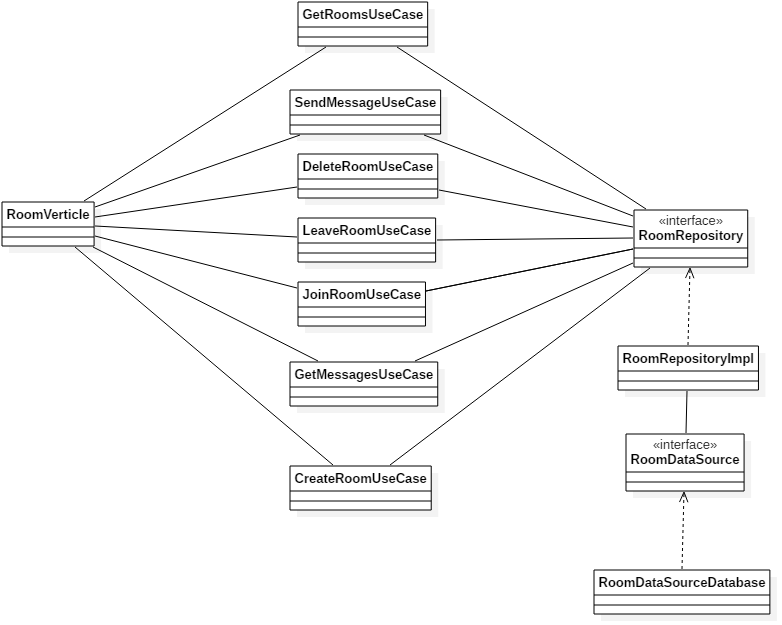
\includegraphics[height=15cm, width=12cm,
		keepaspectratio]{images/RoomServiceClassDiagram.png}
  \caption{Diagramma delle classi del \textit{Room Service} (alcuni casi d’uso sono stati omessi per facilitare la lettura dello schema).}
  \label{fig:room-service-class-diagram}
\end{figure}

\paragraph{Authentication Service}
L' \textit{Authentication Service} è il servizio che si occupa della gestione dell'autenticazione dell'utente e della protezione delle rotte di navigazione per le quali bisogna essere loggato per accedervi. Gestisce la persistenza delle credenziali degli utenti ed offre il servizio di creazione e validazione dei \textit{token}.
La struttura di questo servizio è descritta dal diagramma delle classi in Figura \ref{fig:authentication-service-class-diagram}.
\begin{figure}
  \centering
  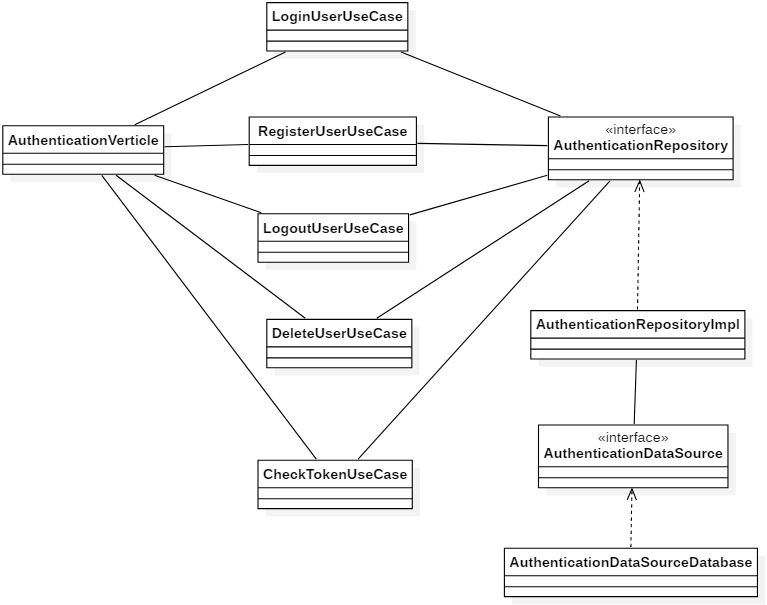
\includegraphics[height=15cm, width=12cm,
		keepaspectratio]{images/AuthenticationServiceClassDiagram.png}
  \caption{Diagramma delle classi dell'\textit{Authentication Service}.}
  \label{fig:authentication-service-class-diagram}
\end{figure}

\paragraph{Heartbeat Service}
L'\textit{Heartbeat Service} è il microservizio che si occupa di monitorare lo stato del client. Questo servizio monitora periodicamente i client connessi al sistema verificando se sono ancora connessi. In questo modo il sistema \textit{Server} riuscirà ad inviare ai vari client le informazioni riguardo lo stato di altri utenti.

\subsubsection{Interazione}
In primo luogo, viene riportata la descrizione della gerarchia dei microservizi che ne regola l'interazione. Infine, vengono presentati alcuni scenari di interazione tra i componenti del sistema.
\paragraph{Gerarchia dei microservizi}
La radice della gerarchia dei microservizi è rappresentata dal \textit{WebApp Service}. Quest'ultimo servizio infatti, funge da entry-point del sistema \textit{Server} e quindi da collante tra \textit{Client} e \textit{Server} (il \textit{Client} contatta sempre il \textit{WebApp Service}).
Il \textit{WebApp Service} a sua volta comunicherà, a seconda della funzionalità richiesta, con il \textit{Room Service}, \textit{Authentication Service} e \textit{User Service}. I servizi \textit{Room} e \textit{User} presentano una dipendenza verso il servizio di \textit{Authentication} poichè per effettuare alcune operazioni è necessario essere autenticati; quindi l'Authentication Service dovrà prima validare il \textit{token} dell'utente richiedente. Come è possibile vedere in Figura \ref{fig:microservices-hierarchy}, il WebApp Service interagisce anche con un \textit{servizio di Heartbeat}. Quest'ultimo è stato pensato per verificare e restituire lo stato di connessione dei \textit{Client} alla \textit{Web Application}.

\begin{figure}
    \centering
  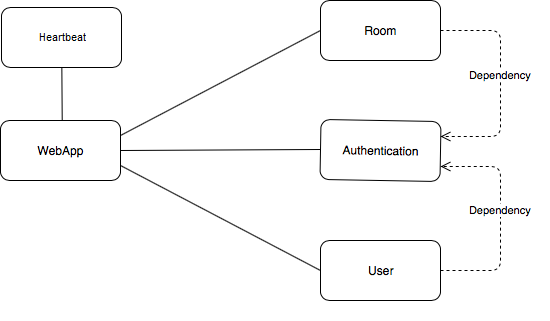
\includegraphics[width=\linewidth]{images/MicroserviceHierarchy_with_heartbeat.png}
  \caption{Gerarchia dei microservizi identificati per il back-end.}
  \label{fig:microservices-hierarchy}
\end{figure}

\subsection{Database}
Il modello scelto per il design del \textit{Database} è quello \textit{relazionale} poichè la natura dei dati è prevalentemente di tipo strutturata.
Per ogni microservizio che necessita di persistenza, è stato modellato uno \textit{schema E/R} che ne descriva la struttura dei dati. Secondo tale modello infatti, ogni servizio gestirà il proprio database che implementerà il relativo schema relazionale.
Di seguito vengono riportati gli schemi E/R dei servizi che utilizzano un \textit{Database}.

\subsubsection{Room Service DB}
Il database del \textit{Room Service} presenta 4 relazioni: 
\begin{itemize}
    \item \textit{User}: identificata dal solo \textit{username}. Uno \textit{User} può partecipare a più stanze e può essere il creatore di una stanza.
    \item \textit{Participation}: identificata dalla \textit{data di unione} ad una stanza, da un \textit{utente} e da una \textit{stanza}. Una partecipazione riguarda solamente un utente ed una stanza. Ad una partecipazione possono essere associati 1 o più messaggi.
    \item \textit{Message}: identificata da una partecipazione e da un timestamp. Presenta l'attributo \textit{content} che rappresenta il testo del messaggio. Ad ogni messaggio è associato una sola partecipazione.
    \item \textit{Room}: identificata dal solo \textit{nome della stanza}. Ogni stanza ha un solo creatore e può essere associata ad una o più partecipazioni.
\end{itemize}

\begin{figure}
    \centering
  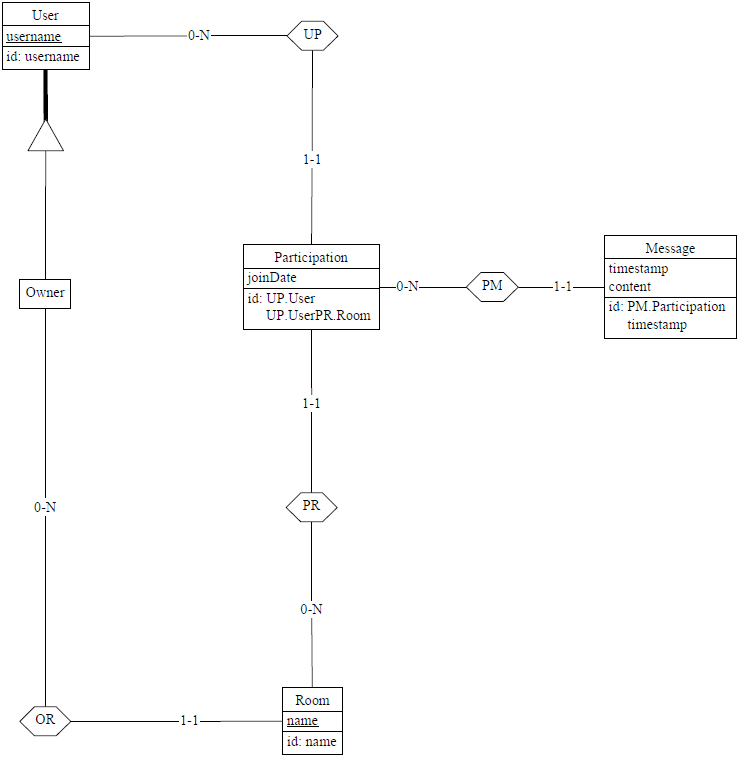
\includegraphics[height=15cm, width=12cm,
		keepaspectratio]{images/RoomServiceER.PNG}
  \caption{\textit{Schema E/R} del Database gestito dal \textit{Room Service}.}
  \label{fig:room-service-er-schema}
\end{figure}
\begin{figure}
    \centering
  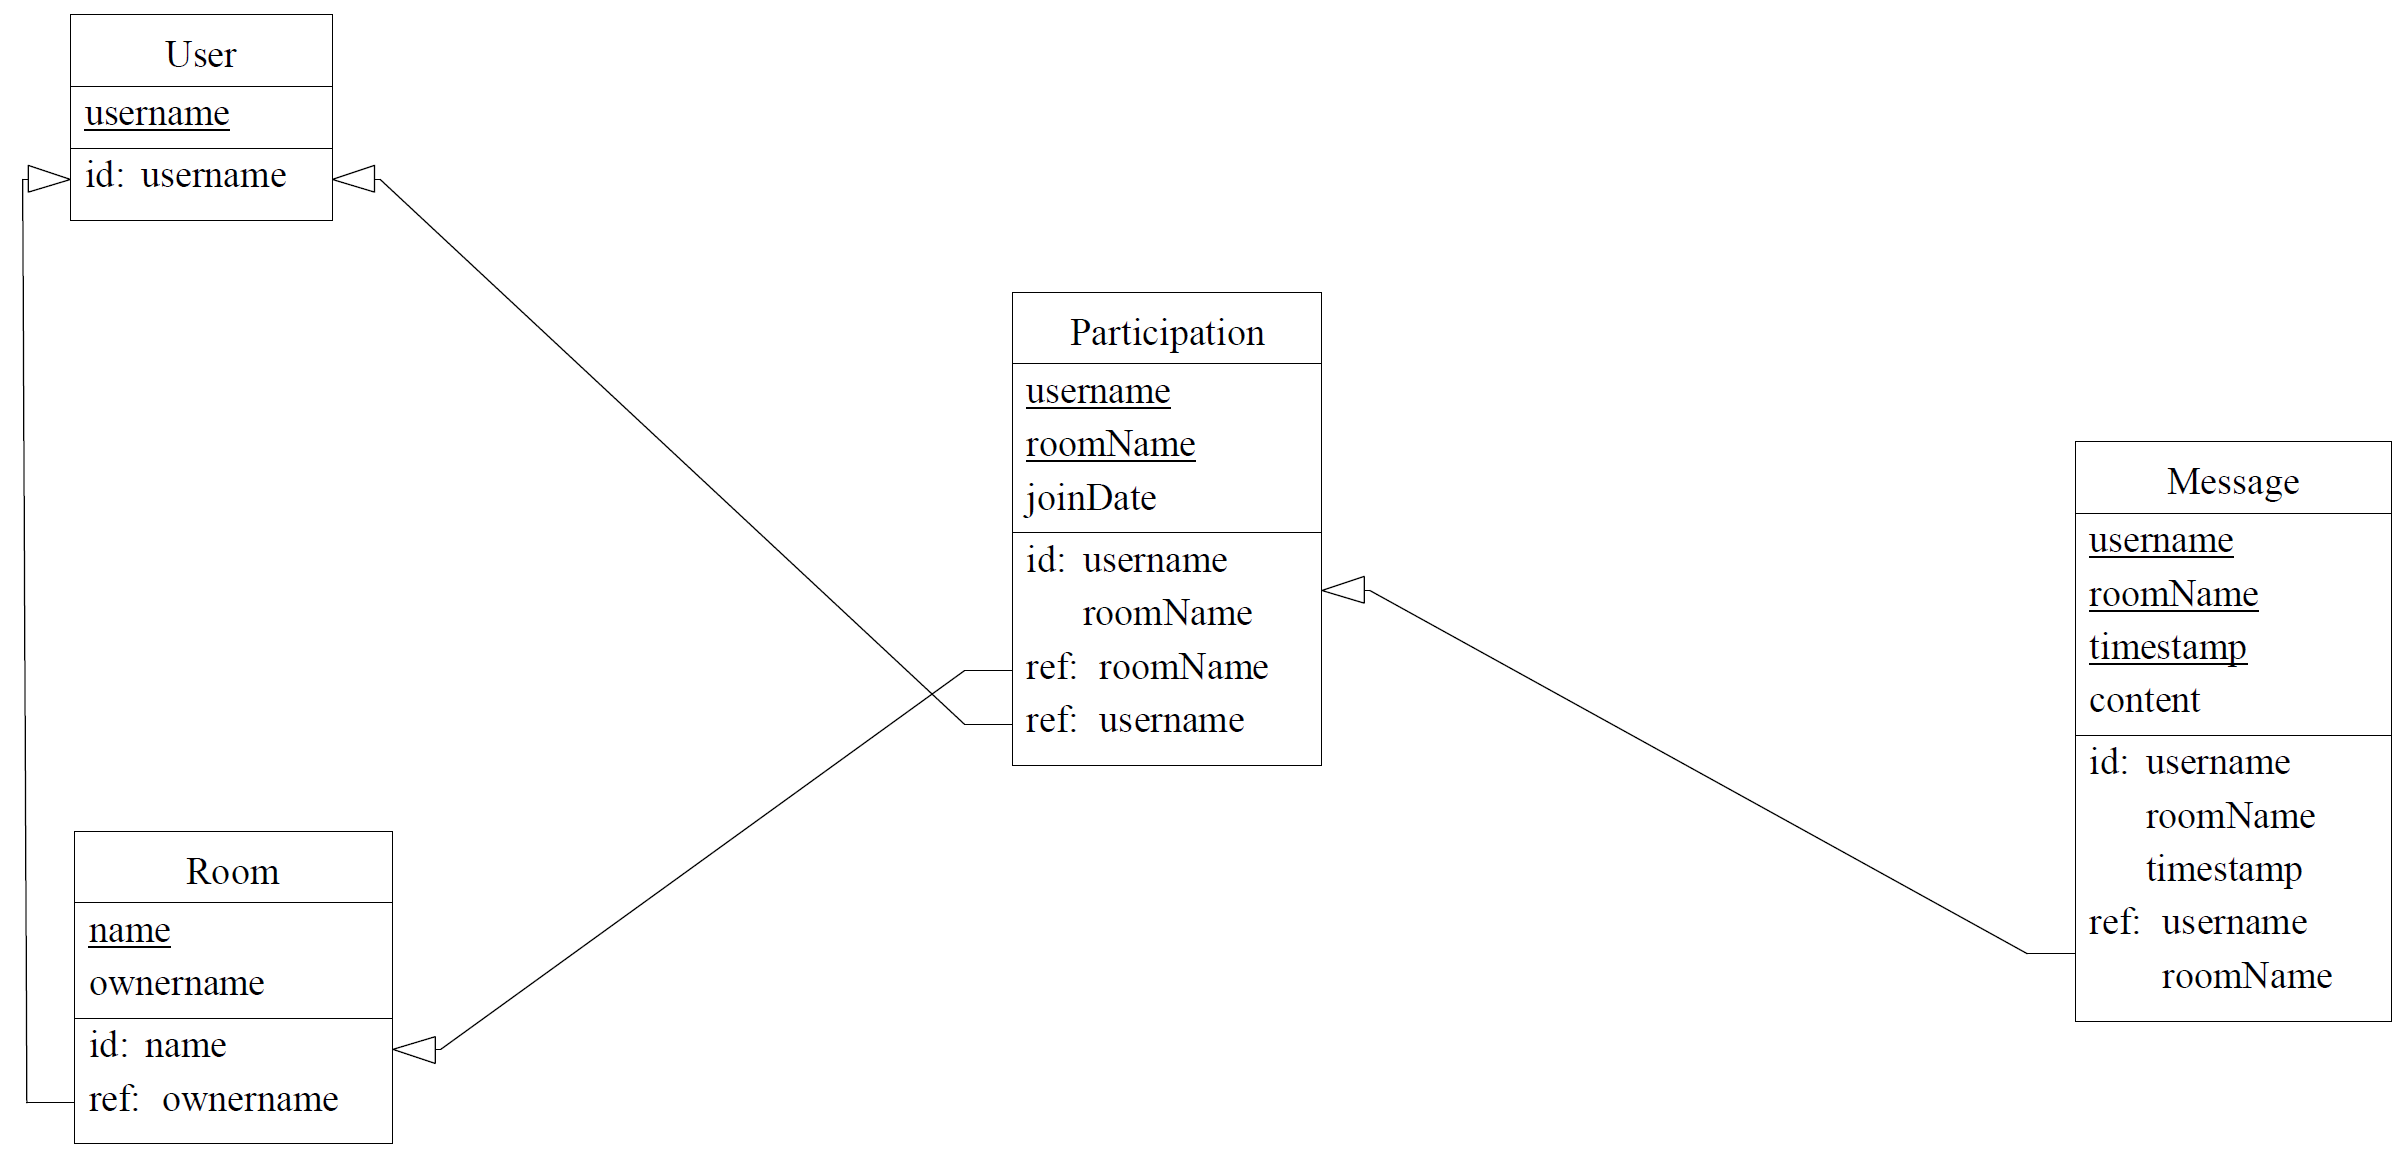
\includegraphics[height=15cm, width=12cm,
		keepaspectratio]{images/RoomServiceDBLogic.png}
  \caption{\textit{Schema logico} del Database gestito dal \textit{Room Service}.}
  \label{fig:room-service-logic-schema}
\end{figure}


\subsubsection{User Service DB}
Il database dello \textit{User Service} presenta una singola relazione \textit{User}. Essa è identificata dallo \textit{username} dell'utente ed è caratterizzata da: 
\begin{itemize}
    \item Nome
    \item Cognome
    \item Biografia
    \item Flag di visibilità
    \item Ultimo accesso
\end{itemize}
\begin{figure}
  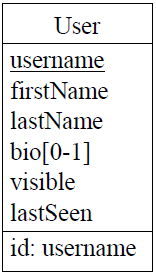
\includegraphics[width=5cm, height=3cm, keepaspectratio]{images/UserServiceER.PNG}
  \centering
  \caption{\textit{Schema E/R} del Database gestito dal \textit{User Service}.}
  \label{fig:user-service-er-schema}
\end{figure}

\newpage
\subsubsection{Authentication Service DB}
Il database dell'\textit{Authentication Service} presenta 2 relazioni: 
\begin{itemize}
    \item \textit{User}: identificato dallo username. È caratterizzata dall'attributo rappresentante la \textit{password} dell'utente. Ad ogni utente possono corrispondere uno o più token invalidi. Quest'ultimi infatti, hanno una scadenza e possono comunque essere invalidati dall'\textit{Authentication Service}. 
    \item \textit{InvalidToken}: identificata dalla stringa del token stesso. Presenta l'attributo corrispondente alla data di scadenza del token.
\end{itemize}

\begin{figure}
  \centering
  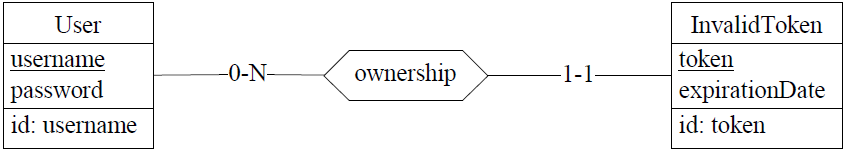
\includegraphics[height=15cm, width=12cm,
		keepaspectratio]{images/AuthenticationServiceER.PNG}
  \caption{\textit{Schema E/R} del Database gestito dall'\textit{Authentication Service}.}
  \label{fig:authentication-service-er-schema}
\end{figure}
\begin{figure}
  \centering
  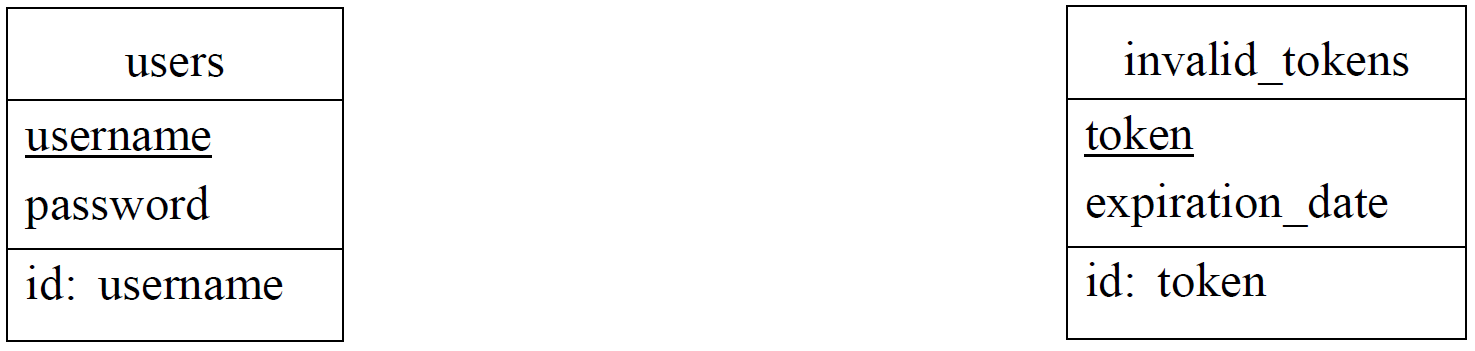
\includegraphics[height=15cm, width=12cm,
		keepaspectratio]{images/AuthenticationServiceDBLogic.PNG}
  \caption{Schema logico del Database gestito dall'\textit{Authentication Service}. L'associazione \textit{ownership} non è stata tradotta in chiave esterna della tabella \textit{invalid\_tokens} in quanto non necessaria; infatti il token intrinsecamente contiene l'informazione relativa allo \textit{username}.}
  \label{fig:authentication-service-logic-schema}
\end{figure}

\subsection{Esempi di interazione}
Riportiamo i diagrammi di sequenza riportanti alcuni degli scenari di interazione più interessanti che coinvologono i componenti core del sistema:
\begin{itemize}
    \item \textbf{Login di un utente} (Figura  \ref{fig:login-sequence-diagram})
        \begin{figure}
           \centering 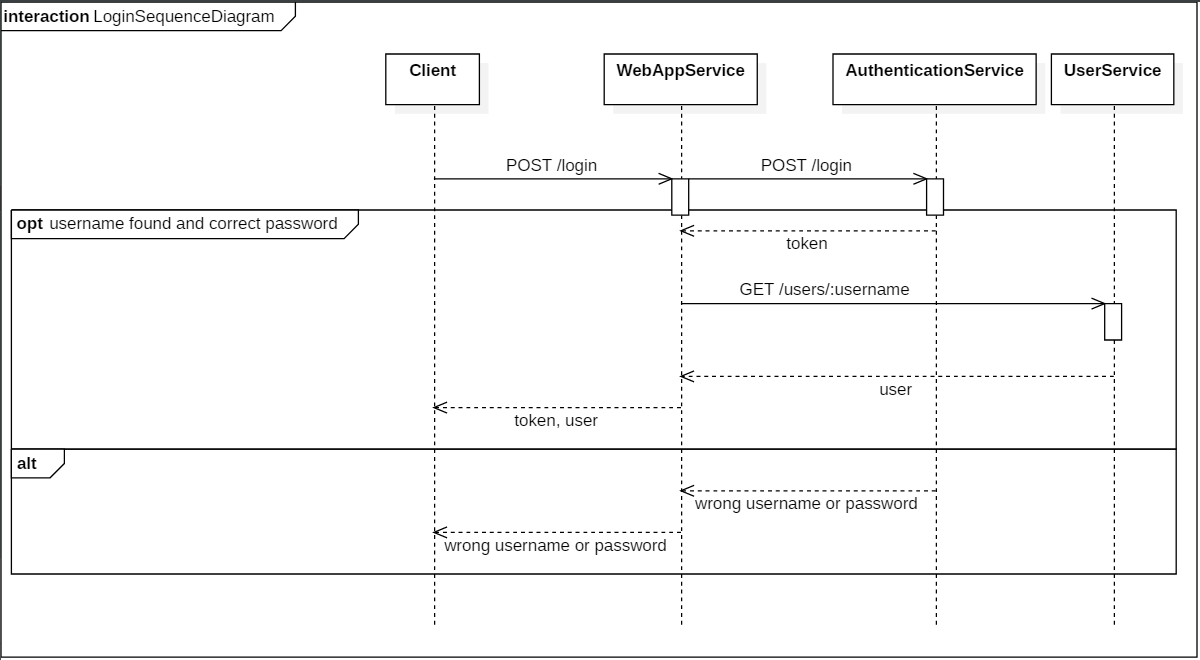
\includegraphics[width=\linewidth]{images/LoginSequenceDiagram.PNG}
            \caption{Diagramma di sequenza del login di un utente.}
            \label{fig:login-sequence-diagram}
        \end{figure}
        
    \item \textbf{Logout di un utente} (Figura  \ref{fig:logout-sequence-diagram})
        \begin{figure}
           \centering 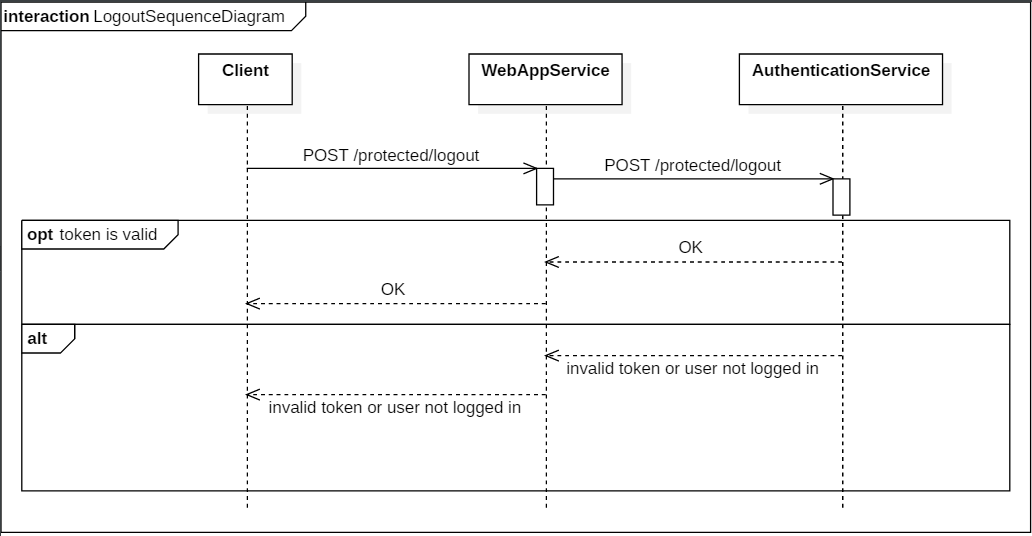
\includegraphics[width=\linewidth]{images/LogoutSequenceDiagram.PNG}
            \caption{Diagramma di sequenza del logout di un utente.}
            \label{fig:logout-sequence-diagram}
        \end{figure}
        
    \item \textbf{Registrazione di un utente} (Figura  \ref{fig:registration-sequence-diagram})
        \begin{figure}
           \centering 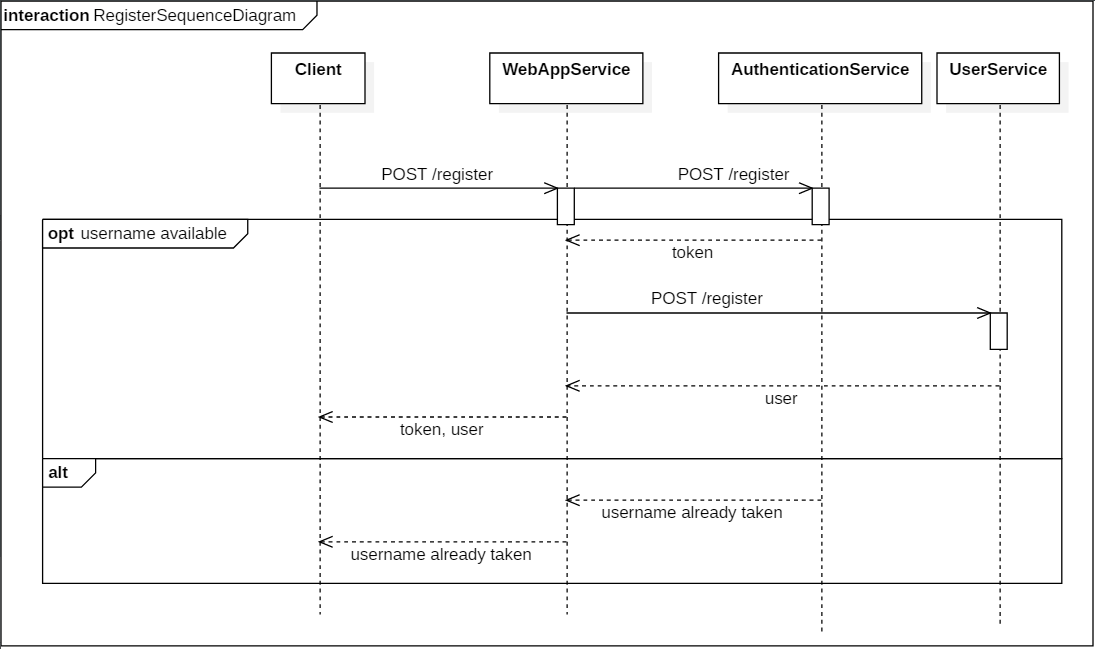
\includegraphics[width=\linewidth]{images/RegistrationSequenceDiagram.PNG}
            \caption{Diagramma di sequenza della registrazione di un utente.}
            \label{fig:registration-sequence-diagram}
        \end{figure}
        
    \item \textbf{Partecipazione ad una stanza} (Figura \ref{fig:join-room-sequence-diagram})
        \begin{figure}
           \centering 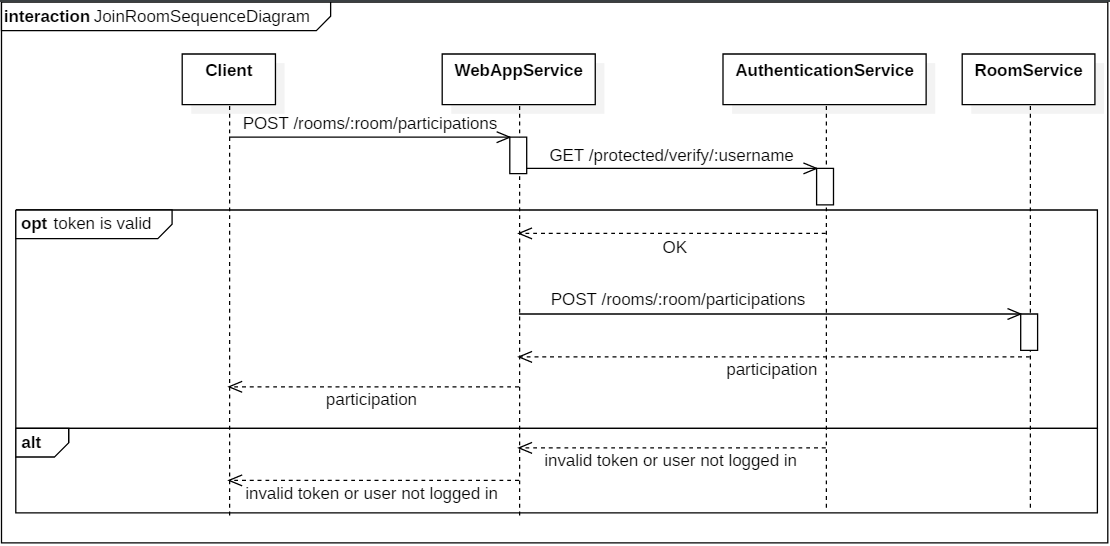
\includegraphics[width=\linewidth]{images/JoinRoomSequenceDiagram.PNG}
            \caption{Diagramma di sequenza dell'unione ad una stanza da parte di un utente.}
            \label{fig:join-room-sequence-diagram}
        \end{figure}
\end{itemize}


\section{Scelte tecnologiche cruciali ai fini architetturali}
\subsection{Vertx}
Vertx è un framework \textit{Event-Driven} poliglotta, utilizzabile per costruire applicazioni reattive sulla JVM. È inoltre non
bloccante, modulare e particolarmente veloce, favorendo così la concorrenza e la scalabilità. 
\\Il seguente è un elenco delle principali funzionalità e componenti sfruttati, resi disponibili da Vertx:
\begin{itemize}
    \item \textit{Verticle}: Vertx permette l'uso di un modello di concorrenza e deployment semplice, scalabile e Actor-like,
    realizzabile facendo uso dei Verticles. Un'applicazione Vertx è formata da uno o più Verticles, i quali possono essere \textit{Standard}, ovvero basati su un event loop, oppure \textit{Worker}, usando così uno dei thread dal Worker Pool, oppure \textit{Multi-threaded worker}, rendendo il codice eseguibile da più threads;
    \item \textit{EventBus}: è il "sistema nervoso" di Vertx, infatti permette diverse parti dell'applicazione di comunicare tra loro tramite scambio di messaggi asincrono, indipendentemente dal loro linguaggio e istanza Vertx in cui eseguono. L'EventBus supporta publish/subscribe e messaggi sia punto a punto sia request-response; esso è suddiviso in canali, potendo così registrare \textit{handlers} e pubblicare messaggi per uno specifico topic. È inoltre possibile creare un "ponte" con Javascript, rendendo dunque possibile l'uso dell'EventBus nei client Web: anche quest'ultima funzionalità è stata utilizzata;
    \item \textit{Clustering}: con questa funzionalità è possibile eseguire un insieme di istanze con capacità di alta disponibilità, dati distribuiti ed un Event Bus distribuito. Ciò è necessario per fare il deploy di Verticles su più istanze di Vertx, permettendo loro di collaborare;
    \item \textit{Vertx-Web}: è un insieme di funzionalità per la costruzione di applicazioni web, facilitando il routing, 
    il passaggio di parametri, la gestione di cookies e sessioni, ecc;
    \item \textit{Service Discovery}: questo componente fornisce un'infrastruttura per pubblicare e scoprire servizi e microservizi, i quali possono contenere risorse di varia natura;
    \item \textit{Vertx-Jdbc}: è un client che permette di interagire con ogni database compatibile con JDBC, usando
    un'API asincrona.
\end{itemize}
\begin{figure}
        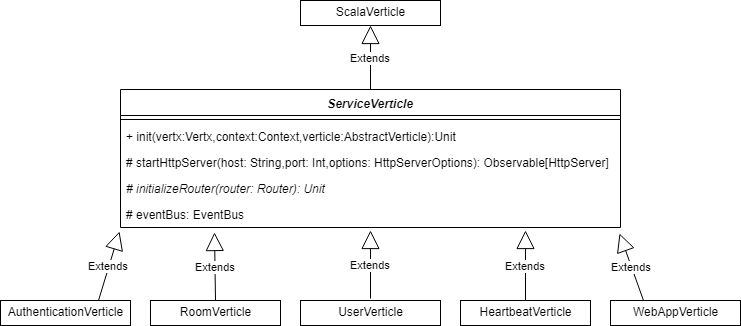
\includegraphics[scale=0.5, center]{images/VerticleClassDiagram.png}
        \caption{Diagramma delle classi che mostra le principali classi del progetto che estendono da \textit{Verticle}.}
        \label{fig:VerticleClassDiagram}
\end{figure}
\begin{figure}
        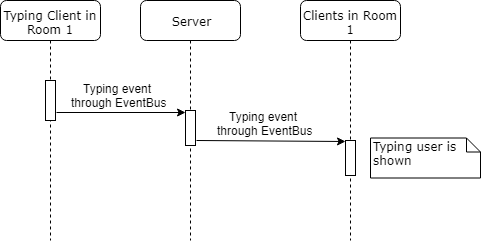
\includegraphics[scale=0.5, center]{images/EventBusSequenceDiagram.png}
        \caption{Diagramma di sequenza di un esempio di uso dell'\textit{EventBus}: l'aggiornamento in real-time dello stato di scrittura di un
        utente in una stanza.}
        \label{fig:EventBusSequenceDiagram}
\end{figure}
\begin{figure}
        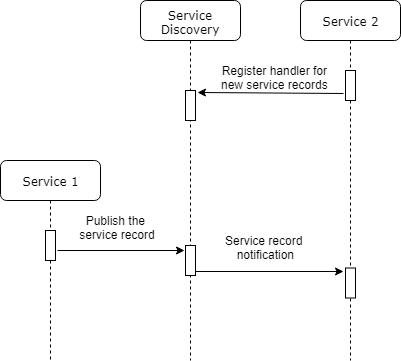
\includegraphics[scale=0.5, center]{images/ServiceDiscoverySequenceDiagram.png}
        \caption{Diagramma di sequenza di un esempio di uso del servizio di \textit{Service Discovery}.}
        \label{fig:ServiceDiscoverySequenceDiagram}
\end{figure}

Vertx è stato dunque scelto per le sue spiccate caratteristiche di velocità, scalabilità e capacità di fornire costrutti di alto livello utili e potenti.

\subsection{Angular}
Angular 2+ (o semplicemente Angular) è una piattaforma open source per lo sviluppo di applicazioni web con licenza \textit{MIT}, evoluzione di \textit{AngularJS}. E' stato sviluppato principalmente da Google, la sua prima release è avvenuta il 14 settembre 2016.
Il linguaggio di programmazione usato per \textit{Angular} è \textit{TypeScript}.

Le applicazioni sviluppate in Angular vengono eseguite interamente dal web browser dopo essere state scaricate dal web server. Questo comporta il risparmio di numerose richieste che dovrebbero essere altrimenti effettuate ogni volta che c'è una richiesta di azione da parte dell'utente. Il codice generato da Angular gira su tutti i principali web browser moderni quali ad esempio \textit{Chrome}, \textit{Microsoft Edge}, \textit{Opera}, \textit{Firefox}, \textit{Safari}, ecc.
I vantaggi dell'utilizzo di tale framework sono davvero considerevoli:
\begin{itemize}
    \item \textbf{TypeScript}: Le applicazioni \textit{Angular} sono costruite usando il linguaggio \textit{TypeScript}, un linguaggio costruito sopra JavaScript, che garantisce maggiore sicurezza in quanto supporta tipi (primitive, interfacce, ecc.) in fase di compilazione. Inoltre, aiuta a catturare ed eliminare gli errori in anticipo durante la scrittura del codice o l'esecuzione di attività di manutenzione.
    \item \textbf{UI espressa in modo dichiarativo} tramite l'uso di \textit{HTML}.
    \item \textbf{POJO}: Con Angular, non sono necessarie ulteriori funzioni getter e setter. Dato che ogni oggetto che usa è POJO (Plain Old JavaScript Object), che abilita la manipolazione degli oggetti fornendo tutte le funzionalità JavaScript convenzionali. È possibile rimuovere o aggiungere proprietà dagli oggetti, oltre a eseguire il loop su questi oggetti quando richiesto.
    \item \textbf{Pattern MVC incorporato}: lo sviluppatore \textit{Angular} non deve creare i classici blocchi previsti dall'architettura \textit{MVC} ma deve solo preoccuparsi di suddividere i componenti SW secondo i concetti forniti dal framework.
    \item \textbf{Struttura modulare}: realizzata tramite la divisione del SW in \textit{components}, \textit{services} e \textit{templates}. In Figura \ref{fig:angular-chat-service-dependencies-diagram} si può vedere un esempio di servizio \textit{Angular}. In particolare è stato scelto di rappresentare la struttura e le dipendenze del \textit{ChatService}. Si riporta, in Figura \ref{fig:angular-room-info-component-dependencies-diagram}, anche un esempio di un componente \textit{Angular}. Nello specifico, è stato rappresentato il componente \textit{room-info}, responsabile delle visualizzazione delle informazioni riguardanti una stanza.
    \begin{figure}
        \centering
        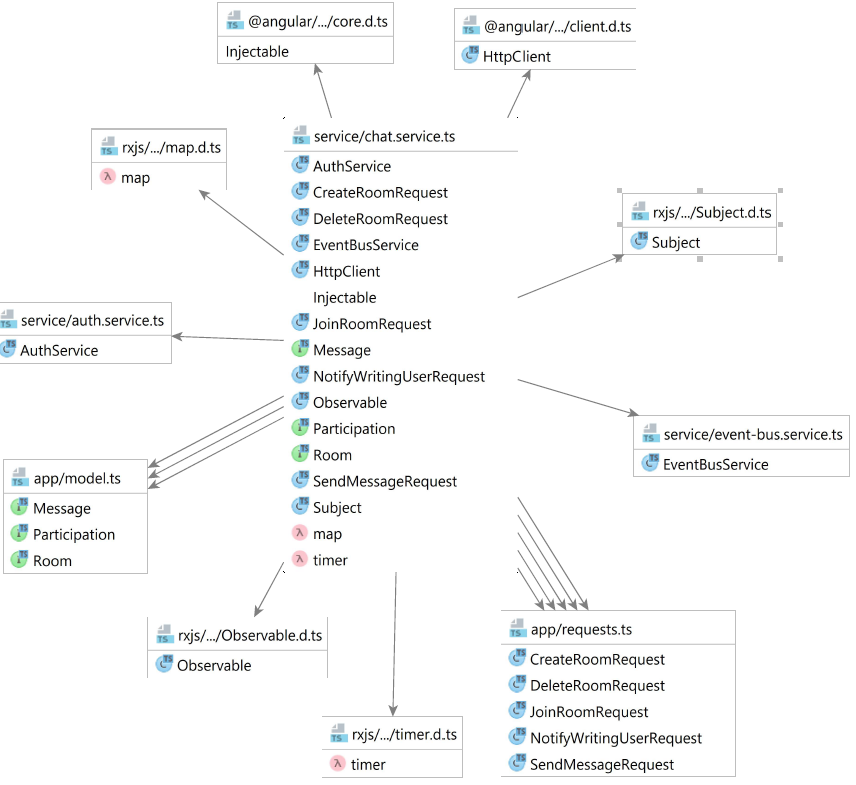
\includegraphics[height=15cm, width=12cm, keepaspectratio]{images/chat-service-dependencies.PNG}
        \caption{Diagramma delle dipendenze del servizio \textit{Angular} \textit{ChatService}.}
        \label{fig:angular-chat-service-dependencies-diagram}
    \end{figure}
    \begin{figure}
        \centering
        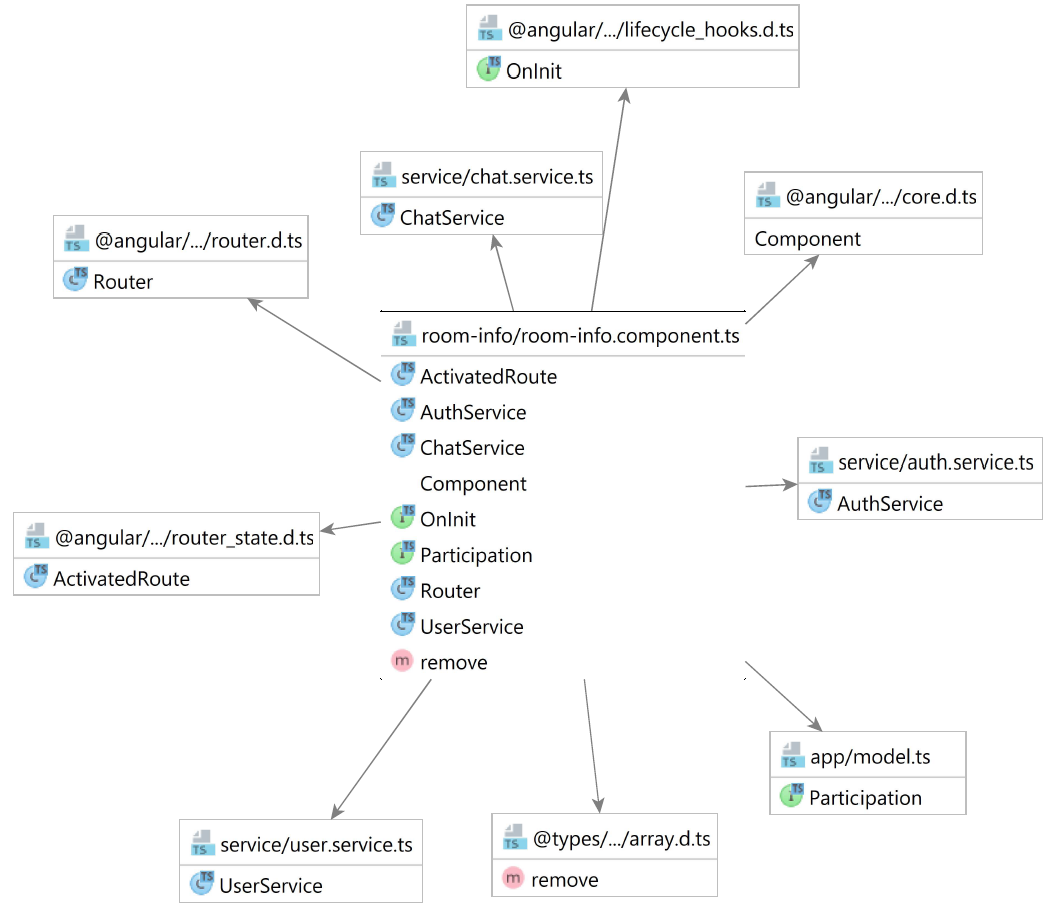
\includegraphics[height=15cm, width=12cm, keepaspectratio]{images/room-info-component-dependencies.png}
        \caption{Diagramma delle dipendenze del componente \textit{Angular} \textit{Room-info}.}
        \label{fig:angular-room-info-component-dependencies-diagram}
    \end{figure}
    \newpage
    \item \textbf{Consistenza del codice} 
        \begin{itemize}
         \item \textbf{Riusabilità}
         \item \textbf{Migliore leggibilità}
         \item \textbf{Facilità di manutenzione}
         \item \textbf{Unit-Testing semplificato}
        \end{itemize}
    \item \textbf{Performance}: in quanto \textit{Angular} mette a disposizione una modalità di deployment detta \textit{Production} nella quale esegue una serie di ottimizzazioni importanti (e.g. minificazione dei file css, js, ecc.).
\end{itemize}
